This section follows up from the design described in \cref{sprint3:design:apps}.
The fragment filled into the fragment container in \lstinline!SettingsActivity! was named \lstinline!AppManagementFragment!.
\lstinline!AppManagementFragment! in turn contains another fragment container, \lstinline!AppsContainer!, where the two fragments derived from \lstinline!AppContainerFragment! will be loaded in - the fragments showing the applications.
Furthermore, \lstinline!AppManagementFragment! implements three buttons in the top of the layout:

\begin{itemize}
\item The \textbf{Giraf} buton loads the \lstinline!GirafFragment! into the fragment container
\item The \textbf{AndroidButton} loads the \lstinline!AndroidFragment! into the fragment container
\item The \textbf{Google Play} button opens the Play Store App. If the apps is not installed on the device, it opens the Play Store in the default browser.
\end{itemize}

The \textbf{Giraf} button and the \textbf{Android} button loads a new fragment into \lstinline!AppsContainer!.
The \textbf{Google Play} button launches the correct intent - The Play Store application or opening the native brower with the Play Store url.

\vagner{finish thissection}
\paragraph{AppManagementFragment}

 and how it loads \lstinline!GirafFragment! and  \lstinline!AndroidFragment!.

A requirement from Sprint 2 was a pane in settings, where it can be set up which applications each user has access to.
 \lstinline!SettingsActivity! loads fragments into its container, but because "Apps" should distinguish between \giraf and other Android applications, an additional fragmentcontainer needs to be inserted.
 The idea can be seen visualized in \cref{fig:settingsappfragments}.
 
\begin{figure}[h]
\centering
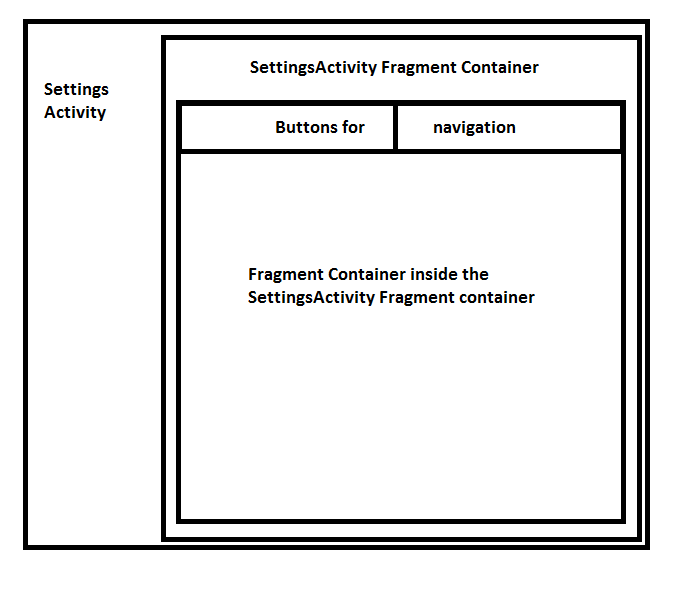
\includegraphics[width=\textwidth, height=3in, keepaspectratio=true] {SettingsActivity.png}
\caption{The organization of \lstinline!SettingsActivity! when inside the "Apps" pane. Since we need to distinguish between \giraf and Android applications, nested fragment containers are used.}
\label{fig:settingsappfragments}
\end{figure}

Because the \giraf and Android pane fragments will contain many of the same variables, these should inherit all shared information from a superclass, consequently reducing redundancy and clarifying how the two fragments are different.

Finally, the navigation buttons inside the \lstinline!SettingsActivity! fragment container should also have a button opening the Google Play Store, so the user can download additional Android applications, if desired. 
Firstly, we researched how to use the inbuilt API for Google Services  to open the Play Store in this way.
However, there were some problems with the API when attempting to implement.
Furthermore, it was discovered that the API is intended to be used for syncronization with Google+, Google Drive and Google Games.
Therefore, we ultimately chose to open the Play Store as a separate activity.\vagner{Please read this and refactor it.}

\vagner{Once again, remember that this is Sprint 3 and should therefore only be the things included in sprint 3!}

| * | 1973797 (3 weeks ago) tonaplo@msn.com the basics of the Android settings tab is now working and have been added.\\
| * | 67726e2 (2 weeks ago) tonaplo@msn.com made the app management part of settings able to load in giraf applications. the onclicklistener used is still wrong, however, and launcher will crash if you choose on of them within settings.\\
* | | d3dd946 (2 weeks ago) fmikke11@student.aau.dk added functionality to laod apps from device\\
* | ec951f4 (2 weeks ago) fmikke11@student.aau.dk Renamed AppFragment to AppManagementFragment. The name was needed for a future class\\
* | 2dd77db (2 weeks ago) fmikke11@student.aau.dk added fragment super class to giraf and android fragments\\
* | | a084d86 (2 weeks ago) fmikke11@student.aau.dk Apps in AndroidFragment are now marked instead of started when clicked\\
* | | bf2409a (2 weeks ago) fmikke11@student.aau.dk started working on parsing list of android apps to home activity\\
| * | | ef137e9 (2 weeks ago) tonaplo@msn.com added functionality to add and remove apps from profiles\\
| * | b837ac1 (2 weeks ago) tonaplo@msn.com Adding and removing GIRAF apps is now fully implemented, both in UI and in function\\
* | | 7787e2e (2 weeks ago) fmikke11@student.aau.dk Apps are now sorted alphabetically, and the functionality for adding android apps to the home activity is now working properply\\
* | | | efc77b3 (2 weeks ago) fmikke11@student.aau.dk Apps are now loaded by another thread\vagner{Betyder dette at vi allerede her havde background loaderen implementeret?}

AppContainerFragment